\section{Rindler decomposition}
\FloatBarrier
		\begin{figure}[tbp]
			\begin{center}
				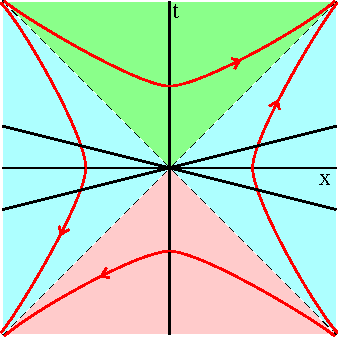
\includegraphics[scale=1]{boost}
				\caption{The \textbf{Rindler decomposition} of \textbf{Minkowski space}. The blue wedges are the Rindler wedges, the red one is the past wedge and the green one is the future wedge. The straight lines in black are slices of the Rindler time. The \textit{red lines} are the action of the \textit{boost operator} $K_x$.}\label{Rindler}
			\end{center}
		\end{figure}
	Now that we know  what entanglement is, we would also like to know, how much who is entangled with whom. In \textbf{Figure \ref{Rindler}} you can see a method which will help us, to reach that goal, the Rindler decomposition of Minkowski space.
	
	Therefore we split the Hilbert space into a factor $\Hil_L$ that acts on the fields $x<0$ and $\Hil_R$ for $x>0$. And each factor has its own basis of states with which we can decompose the vacuum.
	
	We now introduce the \textit{Lorentz boost\footnote{A Lorentz boost is a rotation-free Lorentz transformation, which is a Galilei-transformation in relativistic.\cite{ARTfliesbach} p.7} operator} $K_x$, which mixes x and t but does not act on the y or z direction. This operator exist in any relativistic QFT and looks in the free massive theory like this:
	\begin{equation}
		K_x = \frac{1}{2} \int \diff^3 x 
		\left[ x (\dot{\phi}^2 + \vec{\nabla} \phi \cdot \vec{\nabla} \phi + m^2 \phi^2) + t\dot{\phi} \partial_x \phi
		\right].
	\end{equation}
	It is not explicitly time-dependent, because if you plug it in Heisenberg's equation of motion the time-dependence of the fields cancels the explicit time dependence. \marginpar{Nachrechnen! (siehe QED übung)} In all four regions i.e. wedges of \textbf{Figure \ref{Rindler}} the action of $K_x$ is well defined. 
	
	So in the right blue wedge this operator is evolving forward in time, which is indicated by the red line with the arrow pointing in the increasing $t$ direction. On the contrary $K_x$ is evolving backwards in time in the left blue wedge, where the arrow on the red line is pointing at decreasing t direction. The upper and lower wedge are again the future and the past region where the action of $K_x$ is spacelike. 
	This figure looks very alike the Kruskal extension in \textbf{Figure \ref{kruskal}} but be careful and don't mix them up.
	\FloatBarrier
	\subsection{Eigenstate and Euklidean path integral in general \checkmark}
	We now introduce the Euclidean path integral because we want to find the eigenstates of the left and right Rindler wedges. 
	
	First of all we have a ground state $\ket{\Omega}$ of $H$ and a vacuum state $\ket{0}$, so we can write for a very long time $T$
	\begin{align*}
		e^{-iHT}\ket{0} &= \sum_n e^{-iE_n T} \ket{n}\braket{n|0} \\
		&= e^{-iE_0 T} \ket{\Omega} \braket{\Omega|0} 
		+ \sum_{n\neq 0} e^{-iE_n T} \ket{n} \braket{n|0}
	\end{align*}
	Now we enclose and get the ground state
	\begin{align*}
		\ket{\Omega} &= \lim\limits_{T \rightarrow \infty} \frac{e^{iE_0 T}}{\braket{\Omega|0}} \,e^{-iHT} \ket{0}
	\end{align*}
	We can define $E_0$ with $H_0\ket{0}=\ket{0}$ so
	\begin{align*}
		\ket{\Omega} &=  \frac{1}{\braket{\Omega|0}} \lim\limits_{T \rightarrow \infty} e^{-iHT} \ket{0}
	\end{align*}
	(see p.86 in \cite{PaS}) But this equation does still tell us nothing about the entanglement. So let's continue: \\
	Let a time-independent field $\phi$%, which is a field configuration at $t=0$,
	act on this ground state:
	\begin{align*} \label{groundstate_phi}
		\braket{\phi|\Omega} &= \frac{1}{\braket{\Omega|0}} \lim\limits_{T\rightarrow \infty} \braket{\phi|e^{-iHT}|0} 
	\end{align*}
	Now use the Euclidean path integral formalism, rotate $t$ about 90$^\circ$ in the complex plane: $t \rightarrow -i t_E$ and choose the early boundary condition $\phi=0$, so that
	\begin{align}
		\braket{\phi|\Omega} \propto \int_{\hat{\phi}(t_E = -\infty)= 0}^{\hat{\phi}(t_E = 0)=\phi} D\hat{\phi}e^{-I_E}
	\end{align}
	with the Euclidean action for a free massive scalar field
	\begin{align}
		I_E[\hat{\phi}] = \frac{1}{2} \int \diff^3x \diff t_E \left[
			(\partial_{t_E}\hat{\phi})^2 
			+ (\vec{\nabla}\hat{\phi})^2
			+ m^2\hat{\phi}^2
		\right]
	\end{align}
	Note that $\hat{\phi}$ compared to $\phi$ is time-dependent.
	
	\subsection{The ground states of the Rindler wedges N}
	But instead of integrating from $t_E= -\infty$ to 0, we choose the range of $\pi$ like in \textbf{Figure~\ref{eucpath}}. In addition our Hilbert space is separated in to $\Hil_L$ and $\Hil_R$ with the fields $\phi_L$ and $\phi_R$ so we write 
	\begin{align}
		\braket{\phi_L \phi_R | \Omega} \propto \braket{\phi_R| e^{-\pi K_R} \Theta| \phi_L}
	\end{align}
	Here the $K_R$ is the operator $K_x$ but in the right Rindler wedge while the operator $\Theta$ is antiunitary\footnote{definition Anti Unitär:} also called CPT and exists in all quantum field theories. It acts on a scalar field in the Heisenberg picture like $\Theta^\dagger \phi(t,x,y,z)\Theta = \phi^\dagger(-t,-x,y,z)$ which gives a map between the to Hilbert spaces.
	\begin{figure}[tbp]
		\begin{center}
			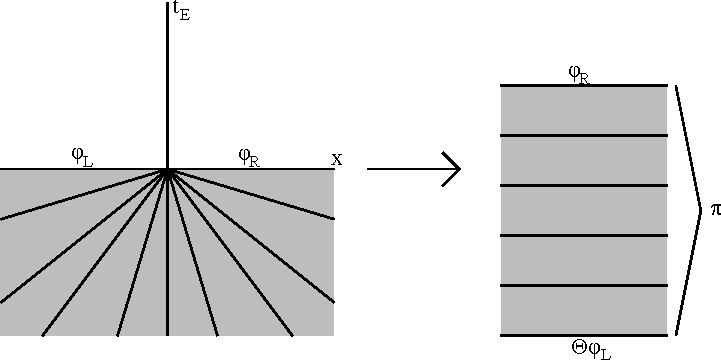
\includegraphics[scale=1]{eucpath}
			\caption{This is the Euclidean path integral representation changing \eqref{groundstate_phi} into a calculable integral, after we choose to integrate over an angle $\pi$. Note that $\varphi_R$ and $\varphi_L$ are the same $\phi$s in the text.}\label{eucpath}
		\end{center}
	\end{figure}
	\subsection{The Unruh temperature N}
	
	\subsection{Entanglement in the Rindler decomposition \checkmark}
	What happens, if we want to cross the $x=0$ surface? For finding that out, we put the system in a mixed state with
		\begin{equation} \label{mixed_state_firewall}
			\rho=\rho_L \otimes \rho_R
		\end{equation}
	instead of having a ground state $|\Omega\rangle$. Here $\rho_L$ and $\rho_R$ are the thermal density matrices, which we get if we trace out the respectively other one in the vacuum $|\Omega\rangle$.
	If the fields are completely discontinuous like in \eqref{mixed_state_firewall} , the gradient term of the Hamiltonian will diverge at $x=0$. If you are an observer in the left or right Rindlers wedge it seems, that you just have vacuum state, but the energy is infinite. 
	
	Its typical field fluctuation is given by $\frac{1}{\epsilon}$ where $\epsilon$ is a short-distance length cutoff. \marginpar{was ist damit genau gemeint?} So it is valid that
		\begin{equation}
			\partial_x \phi|_{x=0} \propto \frac{1}{\epsilon^2}.
		\end{equation}
	Which means, that the gradient term in the Hamiltonian contributes
		\begin{equation}
			\diff x \int \diff^2 y (\partial_x\phi)^2 \propto 
			\epsilon \int \diff^2 y \frac{1}{\epsilon^4} 
			= \frac{A}{\epsilon^3}
		\end{equation}	
	The smaller $\epsilon$ is the bigger becomes the energy and $\epsilon$ is even to the third power.
	 			
	This is called a \textit{firewall}: A huge concentration of energy at $x=0$, that annihilates anybody who tries to jump through the Rindler horizon into the future wedge.
	
	For example the product states $|00\rangle$ and $|11\rangle$ of the states $\frac{1}{\sqrt{2}}
	(|00\rangle \pm |11\rangle)$ which shall both have smooth horizons, should have them too, because of linearity of quantum mechanics. But as we just saw, no product state possibly can have a smooth horizon in QFT. So, for going smoothly through the Rindlers horizon we need not only any entanglement but it must have the \textit{right entanglement} too.